\chapter{Sprint 2 : Gestion des projets et des équipes}

\section*{Introduction}
Le deuxième sprint déploie la couche projet de la plateforme : création et configuration
de projets, gestion des équipes, invitation de membres par email avec token sécurisé,
statuts Kanban personnalisés, et cycle de vie complet des sprints (planification,
démarrage, clôture avec report automatique du backlog).

% ============================================================
\section{Sprint Backlog}

\begin{table}[H]
  \centering
  \caption{Sprint Backlog — Sprint 2}
  \label{tab:backlog_s2}
  \begin{tabularx}{\textwidth}{C{1.2cm}L{5cm}L{2cm}C{2cm}C{1.5cm}}
    \toprule
    \thead{ID} & \thead{User Story} & \thead{Acteur} & \thead{Priorité} & \thead{Points} \\
    \midrule
    \rowcolor{lightgray}
    US-06 & Créer et configurer un projet              & Member & Must   & 5 \\
    US-07 & Inviter des membres par email (7 jours)    & Chef   & Must   & 8 \\
    \rowcolor{lightgray}
    US-08 & Définir des statuts Kanban personnalisés   & Chef   & Should & 5 \\
    US-09 & Créer et démarrer un sprint                & Chef   & Must   & 8 \\
    \rowcolor{lightgray}
    US-10 & Clôturer un sprint avec report du backlog  & Chef   & Should & 5 \\
    \midrule
    \multicolumn{4}{r}{\textbf{Total :}} & \textbf{31} \\
    \bottomrule
  \end{tabularx}
\end{table}

% ============================================================
\section{Conception}

\subsection{Diagramme de cas d'utilisation}

\begin{figure}[H]
  \centering
  \IfFileExists{figures/sprint2_use_case.png}{%
    \includegraphics[width=0.88\textwidth]{figures/sprint2_use_case.png}%
  }{%
    \fbox{\parbox{0.88\textwidth}{\centering\vspace{1.8cm}
      \textbf{[IMAGE A INSÉRER]}\\[0.4em]
      \texttt{figures/sprint2\_use\_case.png}\\[0.3em]
      \textit{Cas d'utilisation : Chef, Member, Admin, Service Email}
    \vspace{1.8cm}}}%
  }
  \caption{Diagramme de cas d'utilisation — Sprint 2}
  \label{fig:uc_s2}
\end{figure}

\subsection{Diagramme de séquence — Invitation email}

\begin{figure}[H]
  \centering
  \IfFileExists{figures/sprint2_sequence_invite.png}{%
    \includegraphics[width=0.90\textwidth]{figures/sprint2_sequence_invite.png}%
  }{%
    \fbox{\parbox{0.90\textwidth}{\centering\vspace{1.8cm}
      \textbf{[IMAGE A INSÉRER]}\\[0.4em]
      \texttt{figures/sprint2\_sequence\_invite.png}\\[0.3em]
      \textit{Séquence invitation : génération token UUID → email → acceptation → rattachement projet}
    \vspace{1.8cm}}}%
  }
  \caption{Diagramme de séquence — Invitation d'un membre par email}
  \label{fig:seq_invite}
\end{figure}

Le flux d'invitation se déroule en deux phases. La phase d'envoi : le chef de
projet soumet l'email et le rôle souhaité → \texttt{ProjectInviteService::invite()}
génère un token UUID, persiste l'invitation avec une expiration à 7 jours, et met
en file d'attente l'email via \texttt{Mail::queue()}. La phase d'acceptation :
l'invité clique sur le lien → le backend valide le token (non expiré, non accepté),
crée l'entrée \texttt{project\_members} avec le rôle défini, et redirige vers le
projet.

\subsection{Diagramme de classes}

\begin{figure}[H]
  \centering
  \IfFileExists{figures/sprint2_class.png}{%
    \includegraphics[width=0.85\textwidth]{figures/sprint2_class.png}%
  }{%
    \fbox{\parbox{0.85\textwidth}{\centering\vspace{1.8cm}
      \textbf{[IMAGE A INSÉRER]}\\[0.4em]
      \texttt{figures/sprint2\_class.png}\\[0.3em]
      \textit{Classes : Project, Sprint, TaskStatus, Team, ProjectInvitation}
    \vspace{1.8cm}}}%
  }
  \caption{Diagramme de classes — Sprint 2}
  \label{fig:class_s2}
\end{figure}

% ============================================================
\section{Réalisation}

\subsection{Liste des projets avec filtres}

\begin{figure}[H]
  \centering
  \IfFileExists{figures/sprint2_08_projects_list.png}{%
    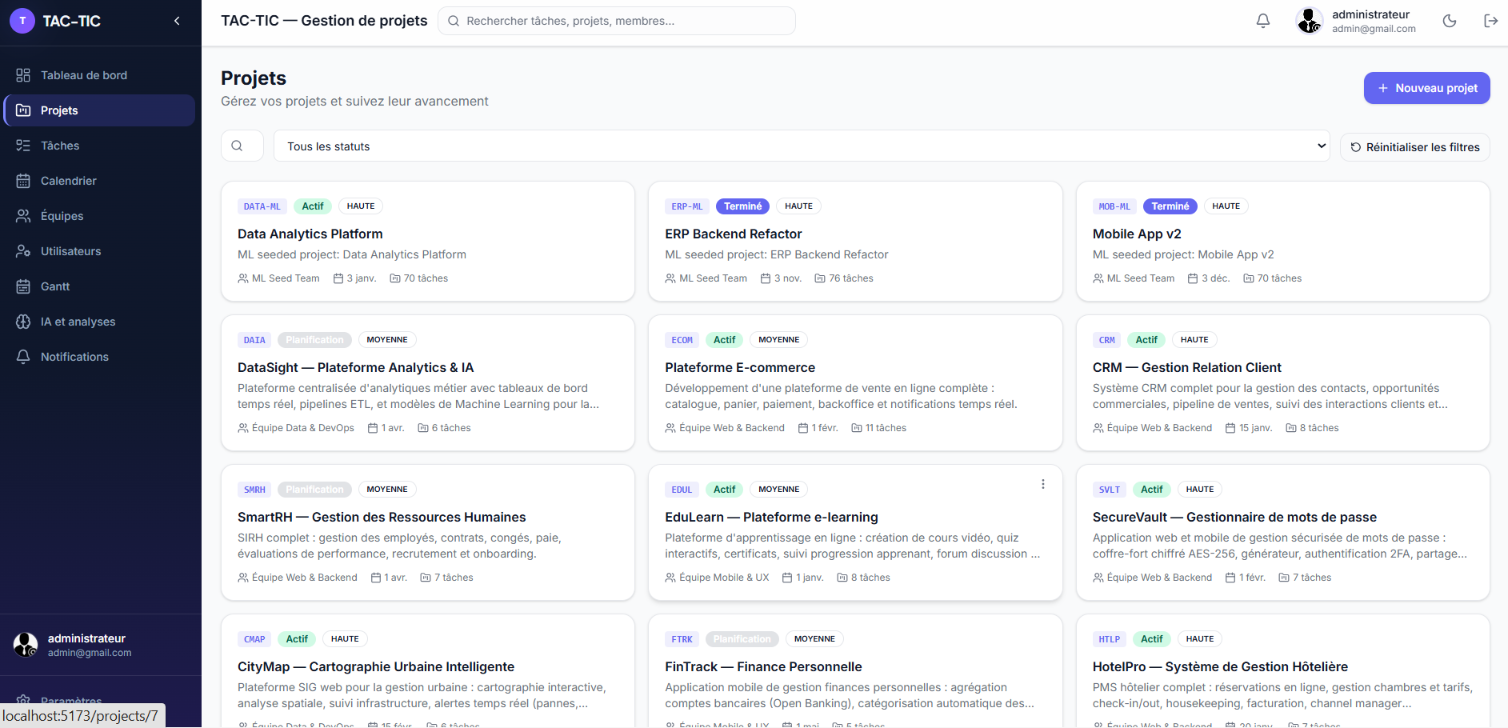
\includegraphics[width=0.88\textwidth]{figures/sprint2_08_projects_list.png}%
  }{%
    \fbox{\parbox{0.88\textwidth}{\centering\vspace{2cm}
      \textbf{[IMAGE A INSÉRER]}\\[0.4em]
      \texttt{figures/sprint2\_08\_projects\_list.png}\\[0.3em]
      \textit{Grille de projets : DataSight, E-commerce, CRM, SmartRH, EduLearn, SecureVault, PFE...}
    \vspace{2cm}}}%
  }
  \caption{Page Projets — Liste avec filtres et statuts colorés}
  \label{fig:ui_projects}
\end{figure}

\subsection{Dashboard projet — KPI et charts}

\begin{figure}[H]
  \centering
  \begin{subfigure}[b]{0.48\textwidth}
    \IfFileExists{figures/sprint2_09_project_kpi.png}{%
      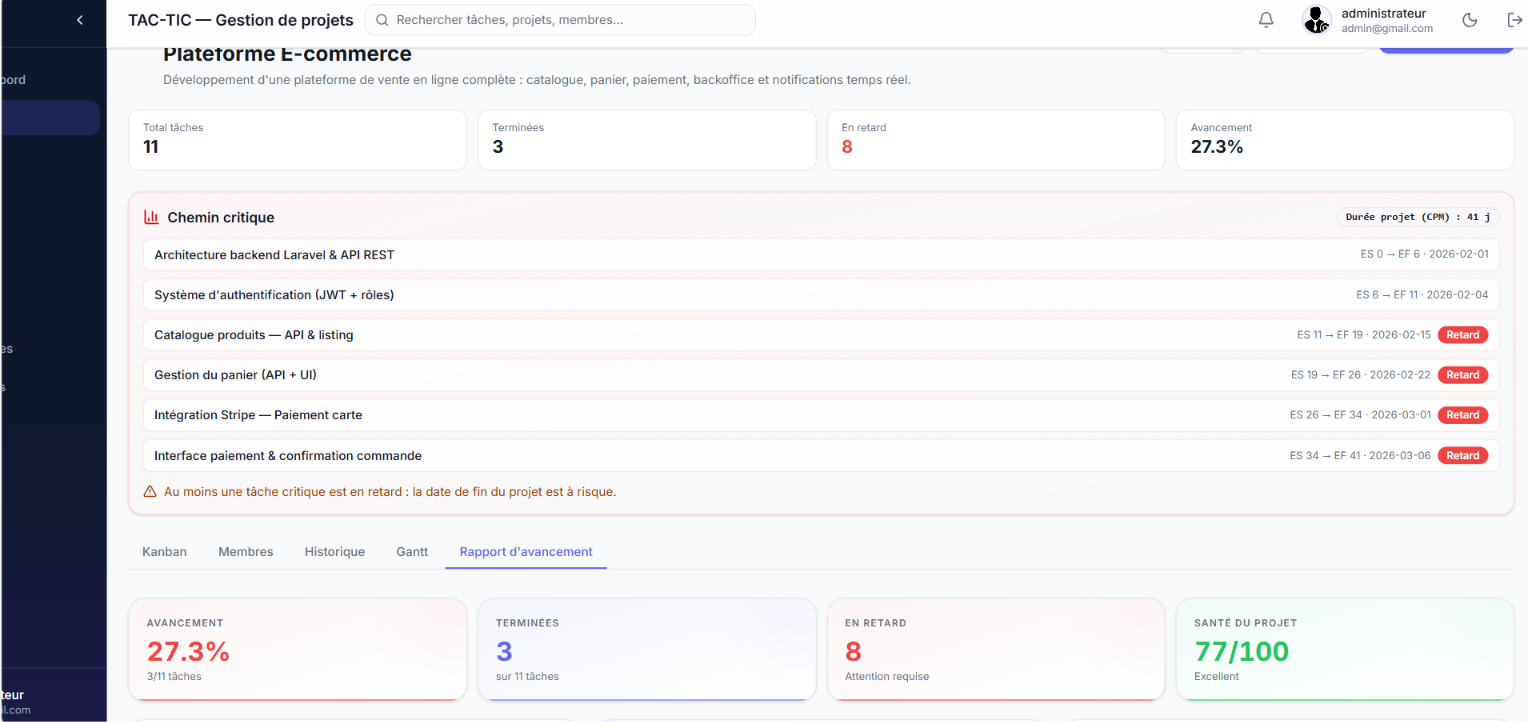
\includegraphics[width=\textwidth]{figures/sprint2_09_project_kpi.png}%
    }{%
      \fbox{\parbox{\textwidth}{\centering\vspace{1.2cm}\small
        \texttt{sprint2\_09\_project\_kpi.png}\\KPI projet\vspace{1.2cm}}}%
    }
    \caption{KPI : avancement, santé, retards}
  \end{subfigure}
  \hfill
  \begin{subfigure}[b]{0.48\textwidth}
    \IfFileExists{figures/sprint2_10_project_charts.png}{%
      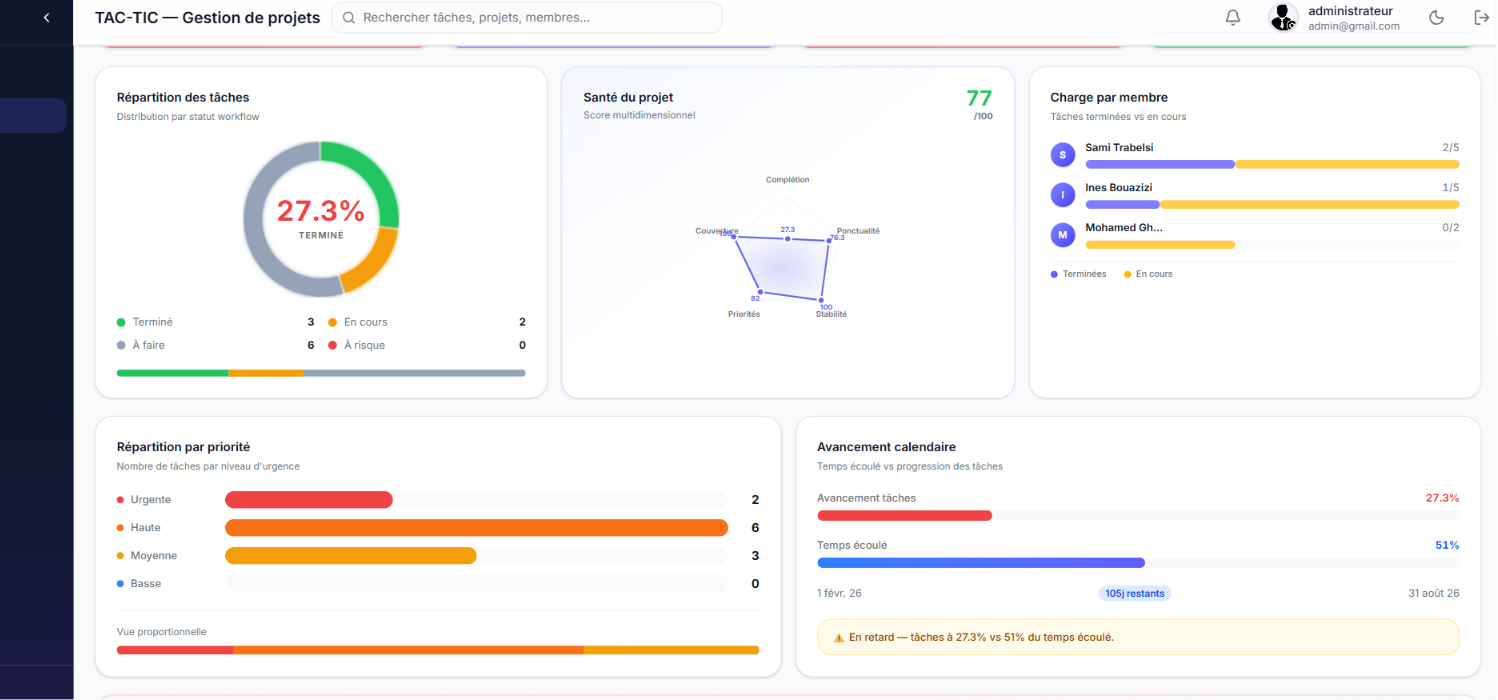
\includegraphics[width=\textwidth]{figures/sprint2_10_project_charts.png}%
    }{%
      \fbox{\parbox{\textwidth}{\centering\vspace{1.2cm}\small
        \texttt{sprint2\_10\_project\_charts.png}\\Charts projet\vspace{1.2cm}}}%
    }
    \caption{Donut statuts, radar santé 5 axes}
  \end{subfigure}
  \caption{Dashboard projet — KPI et visualisations}
  \label{fig:ui_project_dashboard}
\end{figure}

\subsection{Administration utilisateurs et équipes}

\begin{figure}[H]
  \centering
  \begin{subfigure}[b]{0.48\textwidth}
    \IfFileExists{figures/sprint2_11_teams.png}{%
      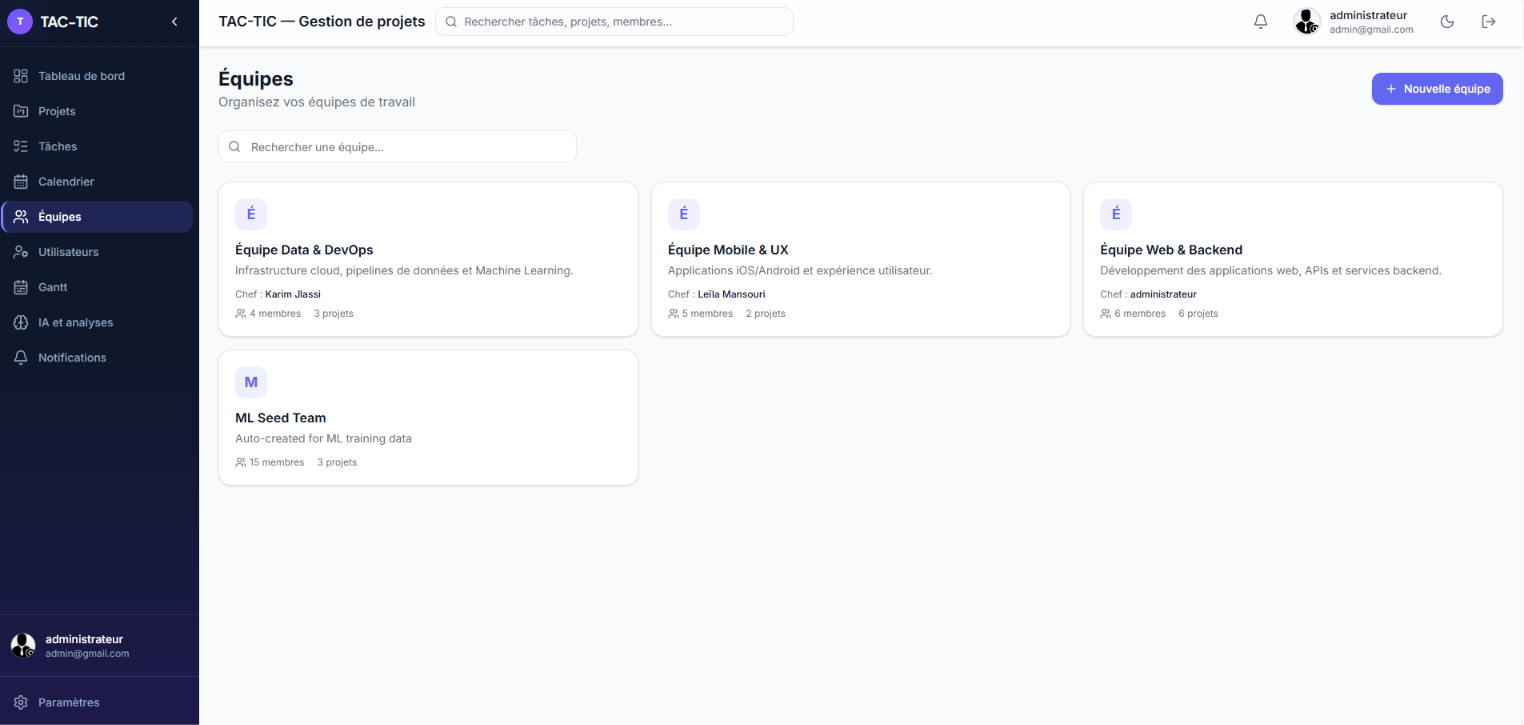
\includegraphics[width=\textwidth]{figures/sprint2_11_teams.png}%
    }{%
      \fbox{\parbox{\textwidth}{\centering\vspace{1.2cm}\small
        \texttt{sprint2\_11\_teams.png}\\Page Équipes\vspace{1.2cm}}}%
    }
    \caption{Page Équipes}
  \end{subfigure}
  \hfill
  \begin{subfigure}[b]{0.48\textwidth}
    \IfFileExists{figures/sprint2_12_users_admin.png}{%
      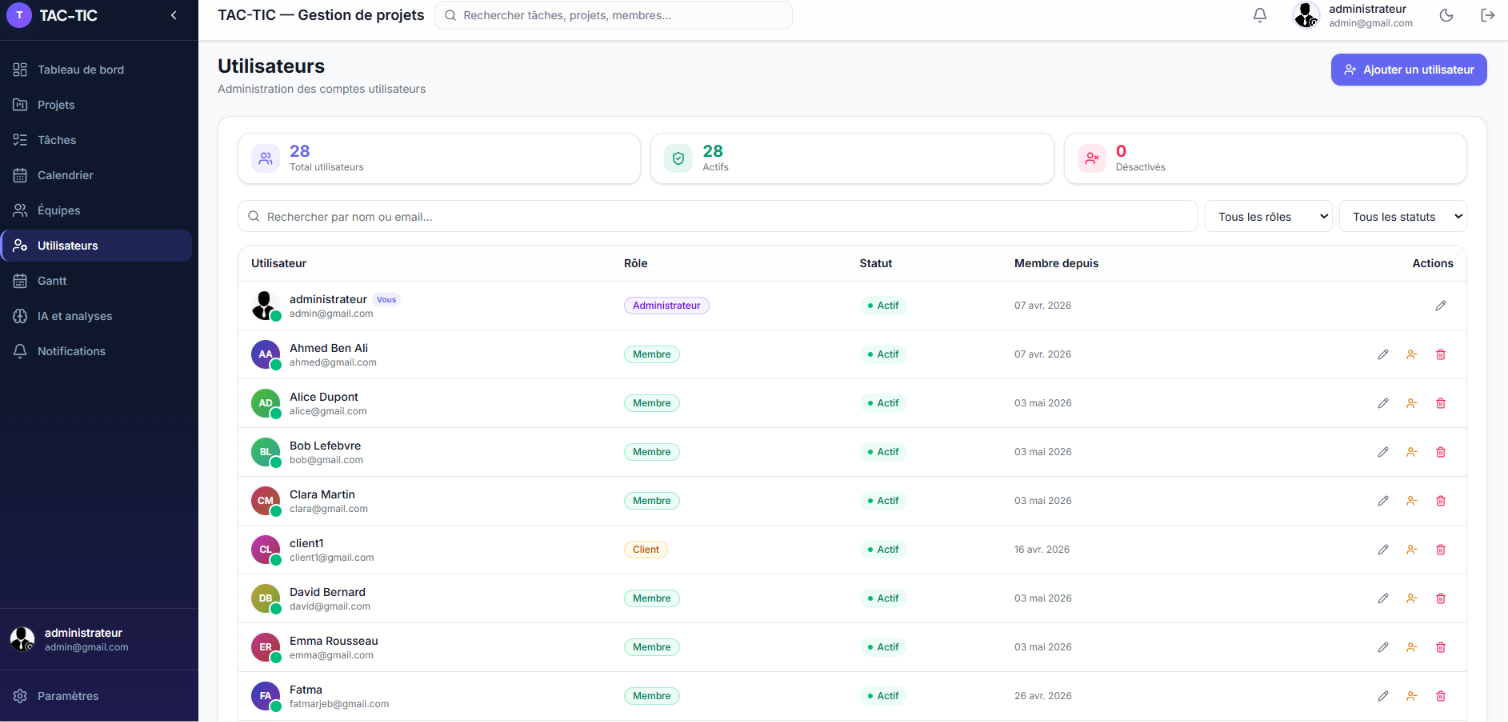
\includegraphics[width=\textwidth]{figures/sprint2_12_users_admin.png}%
    }{%
      \fbox{\parbox{\textwidth}{\centering\vspace{1.2cm}\small
        \texttt{sprint2\_12\_users\_admin.png}\\Gestion utilisateurs\vspace{1.2cm}}}%
    }
    \caption{Administration des utilisateurs}
  \end{subfigure}
  \caption{Gestion des équipes et des utilisateurs}
  \label{fig:ui_teams_users}
\end{figure}



% ============================================================
\section{Tests unitaires}

\begin{lstlisting}[style=phpstyle,caption={Tests unitaires — Projets et sprints (PestPHP)},label={lst:tests_s2}]
it('creates project with valid data', function () {
    $user = User::factory()->create();
    $this->actingAs($user)->postJson('/api/projects', [
        'name'       => 'Test IntelliPM',
        'code'       => 'TIP',
        'priority'   => 'high',
        'start_date' => '2026-02-01',
    ])->assertCreated()
      ->assertJsonFragment(['code' => 'TIP']);
});

it('prevents duplicate active sprints', function () {
    $project = Project::factory()->withActiveSprint()->create();
    $sprint  = Sprint::factory()->make(['project_id' => $project->id]);
    expect(fn() => app(SprintService::class)->start($sprint))
        ->toThrow(HttpException::class, 422);
});

it('returns tasks to backlog on sprint close', function () {
    $sprint = Sprint::factory()->active()->create();
    $task   = Task::factory()->create([
        'sprint_id'       => $sprint->id,
        'workflow_status' => 'in_progress',
    ]);
    app(SprintService::class)->complete($sprint);
    expect($task->fresh()->sprint_id)->toBeNull();
});
\end{lstlisting}

\begin{chapconclusion}
Le sprint~2 a été livré sans dette technique, avec 31 story points délivrés.
Le mécanisme d'invitation email bout-en-bout est opérationnel, incluant la gestion
des expirations à 7 jours et la prévention de doublons. Le rapport d'avancement projet
avec donut de statuts et radar de santé (5 axes) a été très bien reçu lors de la revue.
La gestion des équipes Admin (US-11 bonus) a pu être intégrée dans le temps imparti.
\end{chapconclusion}
